\documentclass{beamer}
\usecolortheme{dove}
\setbeamertemplate{navigation symbols}{}
\usepackage{amsmath,amssymb,amsfonts,amsthm, multicol, subfigure, color}
\usepackage{bm}
\usepackage{graphicx}
\usepackage{tabularx}
\usepackage{booktabs}
\usepackage{hyperref}
\usepackage{pdfpages}
\usepackage{xcolor}
\definecolor{seagreen}{RGB}{46, 139, 87}
\def\independenT#1#2{\mathrel{\rlap{$#1#2$}\mkern2mu{#1#2}}}
\newcommand\indep{\protect\mathpalette{\protect\independenT}{\perp}}
\def\log{\text{log}}
\newcommand\logit{\text{logit}}
\newcommand\iid{\stackrel{\text{iid}}{\sim}}
\newcommand\E{\text{E}}
\newcommand\V{\text{V}}
\renewcommand\P{\text{P}}
\newcommand{\Cov}{\text{Cov}}
\newcommand{\Cor}{\text{Cor}}
\newcommand\doop{\text{do}}


\usepackage{stackrel}
\usepackage{tikz}
\usetikzlibrary{arrows,shapes.arrows,positioning,shapes,patterns,calc}
\newcommand\slideref[1]{\vskip .1cm \tiny \textcolor{gray}{{#1}}}
\newcommand\red[1]{\color{red}#1}
\newcommand\blue[1]{\color{blue}#1}
\newcommand\gray[1]{\color{gray}#1}
\newcommand\seagreen[1]{\color{seagreen}#1}
\newcommand\purple[1]{\color{purple}#1}
\newcommand\orange[1]{\color{orange}#1}
\newcommand\black[1]{\color{black}#1}
\newcommand\white[1]{\color{white}#1}
\newcommand\teal[1]{\color{teal}#1}
\newcommand\magenta[1]{\color{magenta}#1}
\newcommand\Fuchsia[1]{\color{Fuchsia}#1}
\newcommand\BlueGreen[1]{\color{BlueGreen}#1}
\newcommand\bblue[1]{\textcolor{blue}{\textbf{#1}}}
\newcommand\bred[1]{\textcolor{red}{\textbf{#1}}}
\newcommand\bgray[1]{\textcolor{gray}{\textbf{#1}}}
\newcommand\bgreen[1]{\textcolor{seagreen}{\textbf{#1}}}
\newcommand\bref[2]{\href{#1}{\color{blue}{#2}}}
\colorlet{lightgray}{gray!40}
\pgfdeclarelayer{bg}    % declare background layer for tikz
\pgfsetlayers{bg,main} % order layers for tikz
\newcommand\mycite[1]{\begin{scriptsize}\textcolor{darkgray}{(#1)}\end{scriptsize}}
\newcommand{\tcframe}{\frame{
%\small{
\only<1|handout:0>{\tableofcontents}
\only<2|handout:1>{\tableofcontents[currentsection]}}
%}
}

\setbeamertemplate{footline}[frame number]

\setbeamertemplate{navigation symbols}{}

\addtobeamertemplate{footline}{
	\leavevmode%
	\hbox{%
		\begin{beamercolorbox}[wd=\paperwidth,ht=2.75ex,dp=.5ex,right,rightskip=1em]{mycolor}%
			\usebeamercolor[fg]{navigation symbols}\insertslidenavigationsymbol%
		\end{beamercolorbox}%
	}%
	\vskip0.5pt%
}{}




\usepackage[round]{natbib}
\bibliographystyle{humannat-mod}
\setbeamertemplate{enumerate items}[default]
\usepackage{mathtools}

\newcommand{\goalsframe}{\begin{frame}{Learning goals for today}
At the end of class, you will be able to:
\begin{enumerate}
\item Understand propensity score matching and coarsened exact matching
\item Use matching methods to estimate causal effects
\end{enumerate} \vskip .2in
\end{frame}}

\title{Matching Continued}
\author{INFO/STSCI/ILRST 3900: Causal Inference}
\date{3 Oct 2023}

\begin{document}

\maketitle

\goalsframe

\begin{frame}{Matching: so far} 
\bgray{Goal:} Sample Average Treatment Effect on the Treated
{\small
   \[\E(Y^{a = 1} \mid A = 1) - \E(Y^{a = 0}\mid A = 1)\]}
    \vskip .1in

\bgray{Potential Solution:} Create a group of untreated individuals, $\mathcal{M}$, which have a \textbf{similar distribution of $L$} to the treated group
\vskip .1in
 \[\frac{1}{n_m}\sum_{i \in \mathcal{M}} Y_i \approx \frac{1}{n_t}\sum_{i:A_i=1} Y^{a = 0}_i \approx \E(Y^{a = 0}\mid A = 1) \]
\bgray{How:} 
\begin{itemize}
    \item Find untreated unit(s) which are similar to each treated unit\pause
    \item Define ``similar''
\end{itemize}
\end{frame}





\begin{frame}{A common distance metric: Propensity scores}
\only<1-2>{\begin{figure}
\begin{tikzpicture}[x = \textwidth, y = .3\textheight]
\node (a) at (.2, .2) {Job Training};
\node (z1) at (.25, .9) {Age};
\node (z2) at (.4, .95) {Prior Inc};
\node (z3) at (.63, .9) {Education};
\node (y) at (.8, .2) {Income};
\draw[->, thick] (z1) -- (a);
\draw[->, thick] (z1) -- (y);
\draw[->, thick] (z2) -- (a);
\draw[->, thick] (z2) -- (y);
\draw[->, thick] (z3) -- (a);
\draw[->, thick] (z3) -- (y);
\draw[->, thick] (a) -- (y);

\end{tikzpicture}
\end{figure}
}

\only<3->{\begin{figure}
\begin{tikzpicture}[x = \textwidth, y = .3\textheight]
\node (a) at (.2, .2) {Job Training};
\node (z1) at (.25, .9) {Age};
\node (z2) at (.4, .95) {Prior Inc};
\node (z3) at (.63, .9) {Education};
\node (y) at (.8, .2) {Income};
\node (pi) at (.2, .55) {$\pi(\ell_i)$};
\draw[->, thick] (z1) -- (pi);
\draw[->, thick] (z1) -- (y);
\draw[->, thick] (z2) -- (pi);
\draw[->, thick] (z2) -- (y);
\draw[->, thick] (z3) -- (pi);
\draw[->, thick] (z3) -- (y);
\draw[->, thick] (pi) -- (a);
\draw[->, thick] (a) -- (y);

\end{tikzpicture}
\end{figure}
}


\only<2->{
\vspace{1em}
Suppose $\vec{L}$ only affects $A$ through a probability of treatment
\[ \pi_i = \pi(\vec{\ell}_i) = P(A_i = 1 \mid \vec{L} = \vec{\ell}) \]
}


\only<4->{
\vspace{1em}
Conditional exchangeability holds given $\pi(\ell_i)$
}

\end{frame}



\begin{frame}{Why propensity scores are nice} \pause

\begin{itemize}
\item Can match on propensity scores directly instead of $L$\pause
\begin{itemize}
\item Easy to reason about \pause
\item Can directly visualize the univariate matches
\end{itemize} \pause
\item Intuitive: Prioritizes covariates that predict treatment
\item Mathematical guarantees on average \pause
\begin{itemize}
    \item If our DAG is correct \pause 
    \item If our matches are good \pause
    \item We should \textbf{on average} get a matched group which looks like the the treatment group
    \[P(L \mid \pi_i, A_i = 1) = P(L \mid \pi_i, A_i = 0)\]
\end{itemize}
\end{itemize}

\end{frame}




\begin{frame}{A common distance metric: Exact matching}
\pause
   
\begin{itemize}
\item Ideally, we find an exact match for each treated unit
\end{itemize} \vskip .1in
$$
d(i,j) = \begin{cases}
0 &\text{if }\vec{L}_i = \vec{L}_j \\
\infty &\text{if }\vec{L}_i \neq \vec{L}_j \\
\end{cases}
$$
Often leads to \bblue{no matches at all}
\end{frame}

\begin{frame}{A common distance metric: Coarsened exact matching\footnote{Iacus, S. M., King, G., \& Porro, G. (2012). \bref{https://www.cambridge.org/core/journals/political-analysis/article/causal-inference-without-balance-checking-coarsened-exact-matching/5ABCF5B3FC3089A87FD59CECBB3465C0}{Causal inference without balance checking: Coarsened exact matching.} Political Analysis, 20(1), 1-24.}}

\pause
\begin{itemize}
\item Define $\tilde{\vec{L}}$ to be a coarsened version of $\vec{L}$ \pause
\begin{itemize}
\item Example: Age 15-20, 20-25, 25-30, etc 
\end{itemize} \pause
\item Match exactly on $\tilde{\vec{L}}$
\end{itemize} \pause \vskip .1in
$$
d(i,j) = \begin{cases}
0 &\text{if }\tilde{\vec{L}}_i = \tilde{\vec{L}}_j \\
\infty &\text{if }\tilde{\vec{L}}_i \neq \tilde{\vec{L}}_j \\
\end{cases}
$$
\begin{itemize} \pause
\item Benefit: Very transparent \pause
\item Benefit: Directly targets balance in $L$ \pause
\item Drawback: May not find a good match for all individuals \pause
\end{itemize}
\end{frame}






\begin{frame}{Multivariate distances: Recap}

When matching on multivariate $\vec{L}$, you have to define the distance between each pair of confounder values $\vec\ell_j$ and $\vec\ell_i$
\begin{itemize}
\item Manhattan distance
\item Euclidean distanace
\item Mahalanobis distance
\item Coarsened exact distance
\item Propensity score distance
\end{itemize}
There is no right answer! Depends on the setting.
\pause
\vspace{1em}
\begin{itemize}
\item Propensity scores are most popular
\item Sometimes they are substantively meaningful\pause
\item Balance only occurs on average
\end{itemize}

\end{frame}




\begin{frame}{Evaluate the matched sets}
Whatever method, you should check that it worked
\begin{itemize}
\item Compare means of $\vec{L}$ (propensity scores) across groups
\item Possibly compare interaction cells; e.g., race $\times$ age \pause
\item Visually assess distribution 
\end{itemize}
\end{frame}



\begin{frame}{Overlap}

\begin{itemize}
    \item Lack of overlap may indicate violation of positivity assumption
    \[P(A = a \mid L = \ell) > 0 \text{ for all a} \]
    \item Ex: Sarah has no MD training. Would Sarah earn more money if she were a surgeon?
    \[P(A = \text{Surgeon} \mid \text{No MD}) = 0\]
    \item If no good match exists, could be that $P(A = 0 \mid L = \ell) = 0$
\end{itemize}
\end{frame}


\begin{frame}{Matching: A word of warning\footnote{Sekhon, J. S. (2009). \bref{http://sekhon.berkeley.edu/papers/annualreview.pdf}{Opiates for the matches: Matching methods for causal inference.} Annual Review of Political Science, 12(1), 487-508.}} \pause

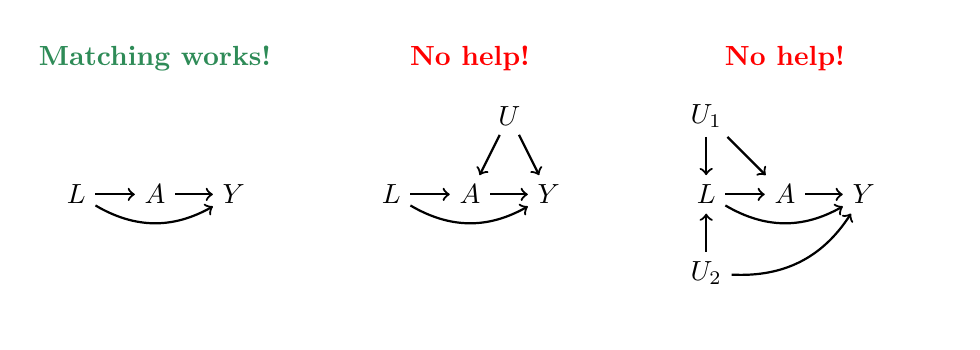
\begin{tikzpicture}
\node at (11,-1.5) {};
\node at (-.5,2) {};
\node (l) at (0,0) {$L$};
\node (a) at (1,0) {$A$};
\node (y) at (2,0) {$Y$};
\draw[->, thick] (l) -- (a);
\draw[->, thick] (l) to[bend right] (y);
\draw[->, thick] (a) -- (y); \pause
\node[anchor = north, seagreen, font = \bf] at (1,2) {Matching works!}; \pause
\node[anchor = north, red, font = \bf] at (5,2) {No help!};
\node (l) at (4,0) {$L$};
\node (a) at (5,0) {$A$};
\node (u) at (5.5,1) {$U$};
\node (y) at (6,0) {$Y$};
\draw[->, thick] (l) -- (a);
\draw[->, thick] (l) to[bend right] (y);
\draw[->, thick] (a) -- (y);
\draw[->, thick] (u) -- (a);
\draw[->, thick] (u) -- (y); \pause
\node[anchor = north, red, font = \bf] at (9,2) {No help!};
\node (l) at (8,0) {$L$};
\node (a) at (9,0) {$A$};
\node (u1) at (8,1) {$U_1$};
\node (u2) at (8,-1) {$U_2$};
\node (y) at (10,0) {$Y$};
\draw[->, thick] (l) -- (a);
\draw[->, thick] (l) to[bend right] (y);
\draw[->, thick] (a) -- (y);
\draw[->, thick] (u1) -- (a);
\draw[->, thick] (u1) -- (l);
\draw[->, thick] (u2) -- (l);
\draw[->, thick] (u2) to[bend right] (y);
\end{tikzpicture}
\onslide<6->{Matching is an estimation strategy.} \\
\onslide<7->{It does not solve identification problems.}\\
\end{frame}




\begin{frame}{Estimating a causal effect}
\begin{itemize}
    \item If we've matched everything well, we can compare the means\pause
    \begin{itemize}
    \item Treated group (with a match)
    \item Matched control group\pause 
    \end{itemize}
    \item We can be extra careful by combining regression + matching
        \begin{itemize}
            \item If everything is perfect, both should be fine on their own\pause
            \item Combining can reduce bias
            \item Reduces model sensitivity\footnote{On the statistical role of inexact matching in observational studies. Guo and Rothenhäusler (2023)}
        \end{itemize}
\end{itemize}
\end{frame}


\begin{frame}{Code}
\Large
Let's try this out in R!
\end{frame}


\goalsframe


\end{document}